%%%%%%%%%%%%%%%%%%%%%%%%%%%%%%%%%%%%%%%%%%
% Engineering problems / LaTeX Template
%		Semester 6
%		Institut d'Optique Graduate School
%%%%%%%%%%%%%%%%%%%%%%%%%%%%%%%%%%%%%%%%%%
%	6N-IntNum-Arduino	/ Embedded System
%%%%%%%%%%%%%%%%%%%%%%%%%%%%%%%%%%%%%%%%%%
%
% Created by:
%	Julien VILLEMEJANE - 30/oct/2024	
%
%%%%%%%%%%%%%%%%%%%%%%%%%%%%%%%%%%%%%%%%%%
% Professional Newsletter Template
% LaTeX Template
% Version 1.0 (09/03/14)
%
% Created by:
% Bob Kerstetter (https://www.tug.org/texshowcase/) and extensively modified by:
% Vel (vel@latextemplates.com)
% 
% This template has been downloaded from:
% http://www.LaTeXTemplates.com
%
% License:
% CC BY-NC-SA 3.0 (http://creativecommons.org/licenses/by-nc-sa/3.0/)
%
%%%%%%%%%%%%%%%%%%%%%%%%%%%%%%%%%%%%%%%%%

\documentclass[a4paper,11pt,titlepage]{article} % The default font size is 10pt; 11pt and 12pt are alternatives

%%%%%%%%%%%%%%%%%%%%%%%%%%%%%%%%%%%%%%%%%%%%%%%%%%%%%%%%%%%%%%%%%%%%%%%%%%%%%%%%%%%%%%%%%%%%%%%%%%%%%%%%%%%%%%%%%%%%%%%%%%%%%%%%%%%%%%%%%%%%%%%%%%%%%%%%%%%%%%%%%%%%%%%%%%%%%%%%%%%%%%%%%%%%%%%%%%%%%%%%%%%%%%%%%%%%%%%%%%%%%%%%%%%%%%%%%%%%%%%%%%%%%%%%%%%%
\usepackage{opto_elec_villemejane}

%%%%%%%%%%%%%%%%%%%%%%%%%%%%%%%%%%%%%%%%%%%%%%%%
%%%%%%%%%%%%%%%%%%%%%%%%%%%%%%%%%%%%%%%%%%%%%%%%
\begin{document}



% Page de garde
\begin{titlepage}

\begin{center}
	\begin{minipage}{2.5cm}
	\begin{center}
		
\includegraphics[width=8cm]{images/Logo-LEnsE.png}
	\end{center}
\end{minipage}\hfill
\begin{minipage}{10cm}
	\begin{center}
	\textbf{Institut d'Optique Graduate School }\\[0.1cm]
    \textbf{Interfaçage Numérique}


	\end{center}
\end{minipage}\hfill


\vspace{4cm}


{\huge \bfseries \textsc{Interfaçage Numérique}} \\[0.5cm]
{\large \bfseries Travaux Pratiques} \\[0.2cm]
Semestre 6

\vspace{2cm}
% Title
\rule{\linewidth}{0.3mm} \\[0.4cm]
{ \huge \bfseries\color{violet_iogs} Arduino et carte Nucléo-STM32 \\[0.4cm] }
\rule{\linewidth}{0.3mm} \\[1cm]

\begin{center}
	
\includegraphics[width=0.15\textwidth]{images/Arduino_Logo.png}

	\bigskip
	
	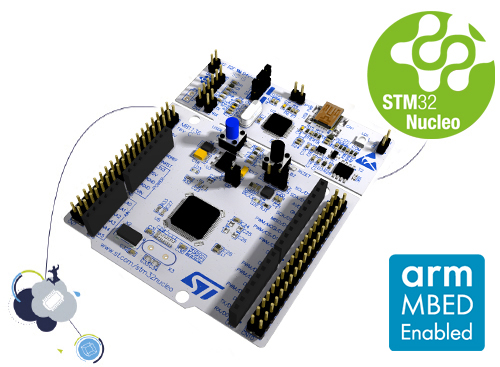
\includegraphics[width=0.4\textwidth]{images/nucleo_board.jpg}	
\end{center}

\vfill

% Bottom of the page
%{\textbf{\large {Année universitaire} 2024-2025}}

\end{center}
\end{titlepage}

\newpage
\pagestyle{empty}
\strut

%%%%%%%%%%%%%%%%%%%%%%%%%%%%%%%%%%%%%%%%%%%%%%%%
%%%%%%%%%%%%%    Intro

\newpage
\pagestyle{plain}
\setcounter{page}{1}

\begin{minipage}[c]{.25\linewidth}
	
\includegraphics[width=5cm]{images/Logo-LEnsE.png}
\end{minipage} \hfill
\begin{minipage}[c]{.4\linewidth}

\begin{center}
\vspace{0.3cm}
{\Large \textsc{Interfaçage Numérique}}

\medskip

6N-047-SCI \qquad \textbf{\large Aide Arduino}

\end{center}
\end{minipage}\hfill

\vspace{0.5cm}

\noindent \rule{\linewidth}{1pt}

{\noindent\Large  \rule[-7pt]{0pt}{30pt} \textbf{Arduino et carte Nucléo-STM32}}

\noindent \rule{\linewidth}{1pt}

\bigskip 

\textit{Ce document est disponible au format électronique sur le site du LEnsE - https://lense.institutoptique.fr/ dans la rubrique Année / Première Année / Interfaçage Numérique S6 / Arduino.}

\noindent \rule{\linewidth}{1pt}

\textit{Vous trouverez également des ressources concernant les \textbf{microcontrôleurs} et les \textbf{systèmes embarqués} à l'adresse suivante :}

\href{https://iogs-lense-training.github.io/nucleo-basics/contents/general.html}{https://iogs-lense-training.github.io/nucleo-basics/contents/general.html}

%%%%%%%%%%%%%%%%%%%%%%%%%%%%%%%%%%%%%%%%%%%%%%%%
%%%%%%%%%%%%%    Arduino
\section{IDE Arduino}

\textbf{Arduino} est une plateforme open-source utilisée pour créer des projets électroniques. Elle est composée de deux éléments principaux : \textbf{une carte matérielle} (contenant un microcontrôleur) et \textbf{un environnement de développement} (IDE Arduino) qui permet de programmer la carte.

\begin{center}
	
\includegraphics[width=0.15\textwidth]{images/Arduino_Logo.png}
\end{center}

Nous nous intéresserons ici qu'à l'environnement de développement qui, après installation d'une extension, permet de programmer d'autres cartes à microcontrôleurs.


%%%%%%%%%%%%%%%%%%%%%%%%%%%%%%%%%%%%%%%%%%%%%%%%
%%%%%%%%%%%%%    Nucleo
\section{Carte Nucleo-STM32}

Les cartes Nucleo sont des \textbf{plateformes de développement} basées sur les \textbf{microcontrôleurs STM32} de \textit{STMicroelectronics}. Elles sont conçues pour faciliter le prototypage et le développement de projets embarqués, similaires aux cartes Arduino, mais elles sont souvent utilisées pour des applications plus complexes et performantes.


\begin{center}
	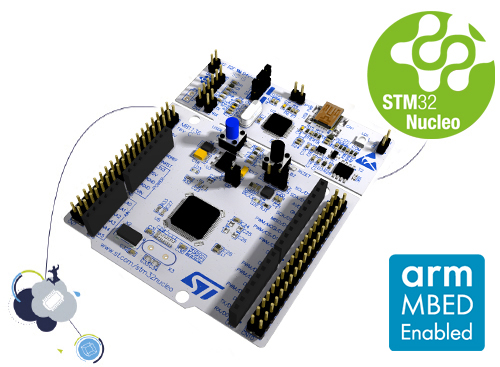
\includegraphics[width=0.3\textwidth]{images/nucleo_board.jpg}
\end{center}

Elles sont équipées d'un débogueur ST-LINK intégré, ce qui permet de programmer et de déboguer le microcontrôleur directement sans matériel additionnel.

\textsl{Le brochage de la carte Nucleo L476RG est fournie en annexe à ce document} : \hyperref[doc:nucleo_pins_476RG]{Brochage Nucléo L476RG}

\textit{Vous trouverez également des ressources concernant les \textbf{microcontrôleurs} et les \textbf{systèmes embarqués} à l'adresse suivante :}

\href{https://iogs-lense-training.github.io/nucleo-basics/contents/general.html}{https://iogs-lense-training.github.io/nucleo-basics/contents/general.html}

\cleardoublepage
%%%%%%%%%%%%%%%%%%%%%%%%%%%%%%%%%%%%%%%%%%%%%%%%
%%%%%%%%%%%%%    Installation des cartes STM32
\section{Installation des cartes STM32}

L'interface de développement \textbf{Arduino}, ainsi que les bibliothèques associées, est populaire pour les projets \textit{Do It Yourself}, l'éducation et le prototypage rapide en raison de sa simplicité et de son accessibilité. Cependant, elle est initialement prévue pour programmer des cartes de type \textbf{Arduino}.

Pour pouvoir bénéficier de l'environnement \textbf{Arduino} pour \textbf{d'autres cartes de prototypage}, il est indispensable d'installer les extensions associées à ces autres cartes.

\textbf{Attention !} La version 2 de l'IDE Arduino est fortement conseillée pour bénéficier des dernières évolutions du langage et de l'interface, ainsi que pour garantir une pleine compatibilité avec les cartes Nucléo.

\subsection{Support des cartes STM32}

Avant de pouvoir utiliser l'environnement Arduino pour programmer des cartes intégrant des microcontrôleurs de type STM32, il faut installer le \textbf{support pour ces microcontrôleurs}.

Dans le menu \textsc{\textbf{Fichiers} / \textbf{Préférences}}, sélectionner le volet \textsc{\textbf{Paramètres}}.

\begin{center}
	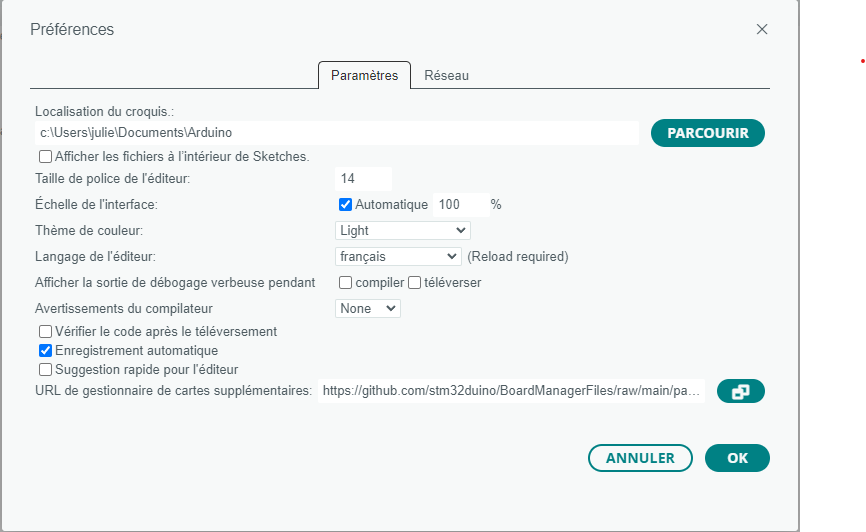
\includegraphics[width=0.75\textwidth]{images/arduino_preferences.png}
\end{center}

Dans la fenêtre \textsc{URL de gestionnaire de cartes supplémentaires}, ajouter l'adresse suivante :

\href{https://GitHub.com/stm32duino/BoardManagerFiles/raw/main/package_stmicroelectronics_index.json}{https://GitHub.com/stm32duino/BoardManagerFiles/raw/main/package\_stmicroelectronics\_index.json}

\begin{center}
	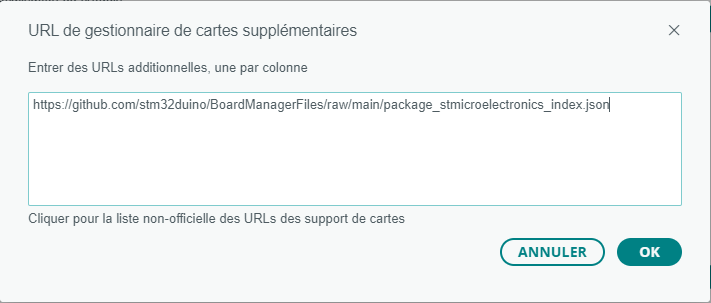
\includegraphics[width=0.6\textwidth]{images/arduino_preferences_url.png}
\end{center}

\subsection{Extension STM32 MCU based boards}

Il faut ensuite télécharger les \textbf{bibliothèques} liées aux cartes intégrant des \textbf{microcontrôleurs STM32} de \textit{STMicroelectronics}.

Aller dans le menu \textsc{\textbf{Outils} / \textbf{Carte} / \textbf{Gestionnaire de carte}}. 

\begin{center}
	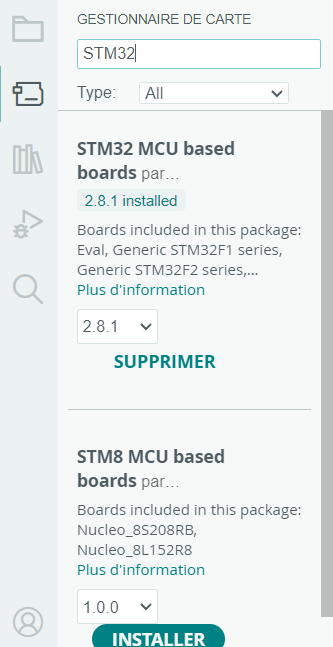
\includegraphics[width=0.3\textwidth]{images/arduino_gestion_cartes.png}
\end{center}

Dans la partie droite de l'interface Arduino, un volet \textsc{\textbf{Gestionnaire de carte}} s'ouvre. Dans la zone de recherche, taper STM32.

Dans la liste, installer alors l'extension : \textbf{STM32 based boards par STMicroelectronics}.

\newpage
\pagestyle{empty}
\strut
\cleardoublepage
\pagestyle{plain}
%%%%%%%%%%%%%%%%%%%%%%%%%%%%%%%%%%%%%%%%%%%%%%%%
%%%%%%%%%%%%%    Premier programme
\section{Premier programme}

Afin de vérifier que toute la chaîne de prototypage est opérationnelle, nous allons nous intéresser à un \textbf{programme de base} permettant de faire \textbf{clignoter une LED} présente par défaut sur la carte Nucléo (c'est également vrai sur les cartes Arduino).

Sélectionner \textsc{\textbf{Fichier} / \textbf{Exemples} / \textbf{01.Basics} / \textbf{Blink}} dans la barre de menu.

Le programme ressemble à celui-ci :

\begin{lstlisting}
void setup() {
  // initialize digital pin LED_BUILTIN as an output.
  pinMode(LED_BUILTIN, OUTPUT);
}

void loop() {
  digitalWrite(LED_BUILTIN, HIGH);  
  	// turn the LED on (HIGH is the voltage level)
  delay(1000);                      
  	// wait for a second
  digitalWrite(LED_BUILTIN, LOW);   
  	// turn the LED off by making the voltage LOW
  delay(1000);                      
  	// wait for a second
}
\end{lstlisting}

\textit{Sur la carte Nucléo la sortie LED\_BUILTIN correspond à la LED nommée LD2.}

Le langage utilisé par l'environnement Arduino est un langage proche du C++. Le programme ainsi écrit doit nécessairement \textbf{être compilé} avant de pouvoir \textbf{être téléversé} sur la carte où il sera ensuite \textbf{exécuté}.

\subsection{Structure du code}

Un programme Arduino (comme tout autre programme embarqué) est constitué de \textbf{deux étapes principales} : 

\begin{itemize}
	\item une \textbf{Initialisation} (fonction \textsl{setup()} pour Arduino) : exécutée une fois à la mise sous tension de la carte ou lors de l'appui sur le bouton Reset.
	\item une \textbf{boucle infinie} (fonction \textsl{loop()} pour Arduino) : exécutée de manière infinie. Cette boucle a pour principale mission, sur un système embarqué, de récupérer les valeurs des entrées, de calculer les valeurs des sorties et de mettre à jour les sorties.
\end{itemize}

\begin{center}
	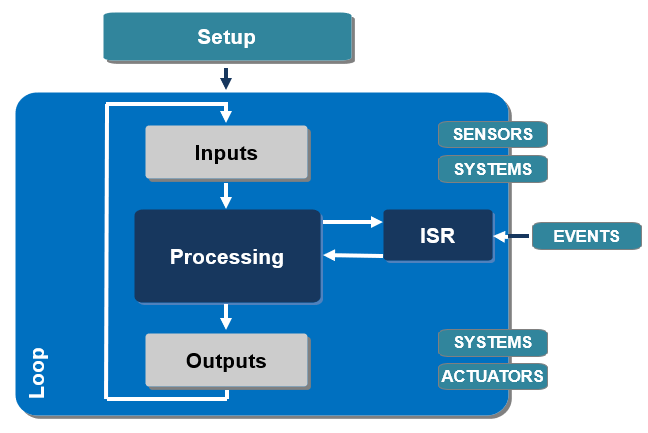
\includegraphics[width=0.4\textwidth]{images/arduino_program_structure.png}
\end{center}

\textit{D'autres étapes sont possibles lorsqu'on autorise le fonctionnement par interruption (voir dans la suite de ce document).}


\subsection{Choix d'une carte}

La compilation d'un tel programme se fait pour une cible particulière. Avant de pouvoir compilé, il est donc nécessaire de préciser sur quel microcontrôleur (ou quelle carte de prototypage) ce code sera exécuté.

Pour cela, dans la barre de menu, sélectionner \textsc{\textbf{Outils} / \textbf{Cartes}}.

Dans le cas d'une carte Nucléo de type L476RG, sélectionner ensuite \textsc{\textbf{STM32 MCU based boards} / \textbf{Nucleo-64}}. Le format pourra changer s'il s'agit d'une autre carte.

\begin{center}
	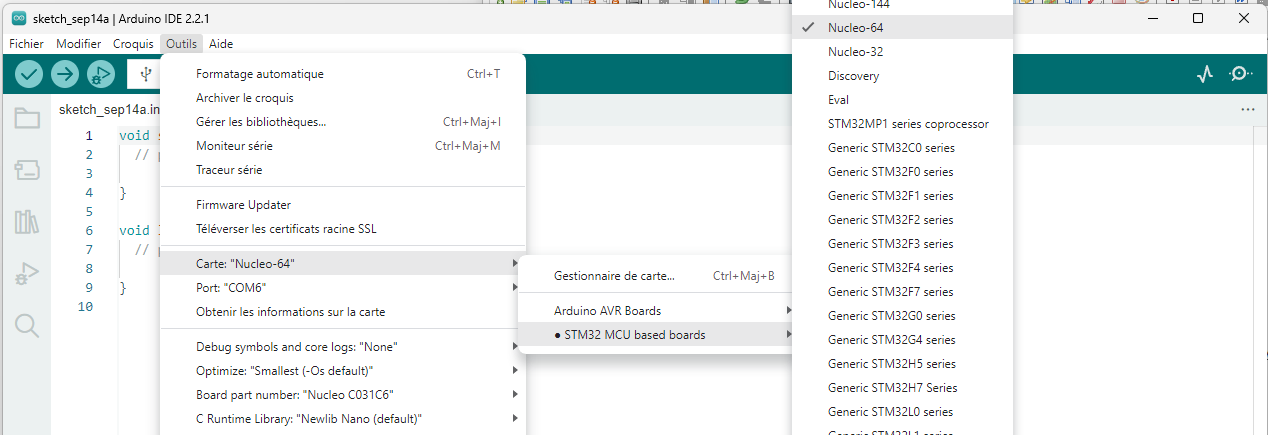
\includegraphics[width=0.75\textwidth]{images/arduino_outils_cartes_nucleo64.png}
\end{center}

Puis, dans le menu \textsc{\textbf{Outils} / \textbf{Board part number}}, sélectionner \textbf{Nucleo L476RG}.

\begin{center}
	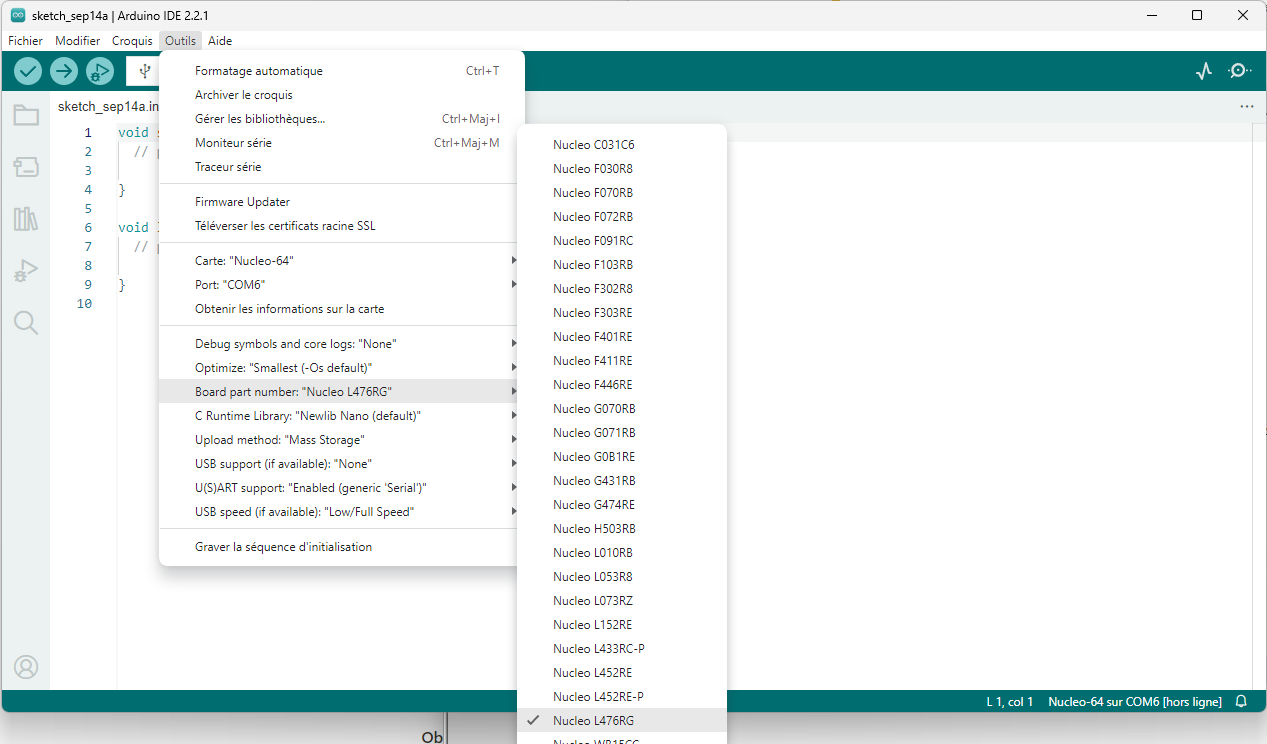
\includegraphics[width=0.75\textwidth]{images/arduino_cartes_nucleo_lxxx.png}
\end{center}

\subsection{Compilation}

Il est maintenant possible de compiler le programme. Pour cela, cliquer sur la première icône de la barre d'action :

\begin{center}
	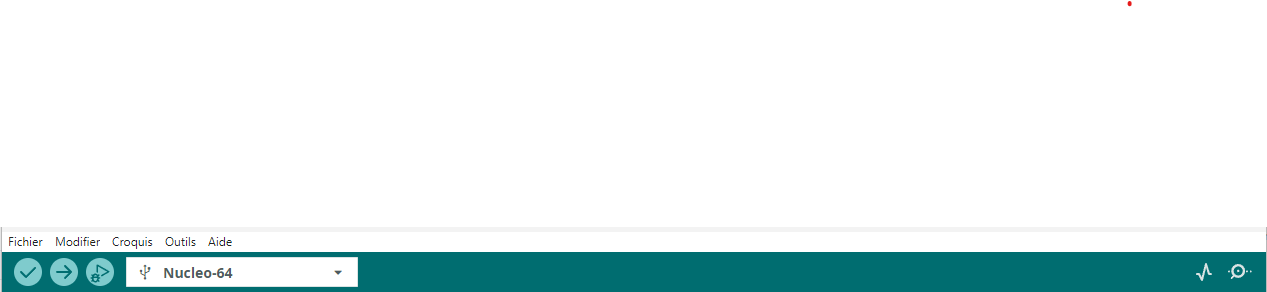
\includegraphics[width=0.9\textwidth]{images/arduino_compile_run.png}
\end{center}

\bigskip


\subsection{Connexion à une carte Nucléo et téléversement}

Il faut ensuite connecter la carte en USB.

Dans la barre des actions possibles sous Arduino, sélectionner le port de communication sur lequel est connectée la carte Nucléo.

\begin{center}
	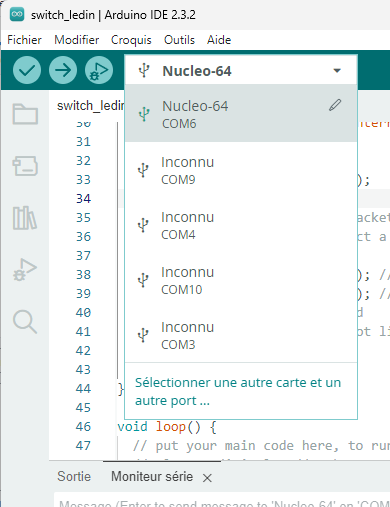
\includegraphics[width=0.4\textwidth]{images/arduino_cartes_nucleo_comXX.png}
\end{center}

Pour téléverser ensuite le code dans la carte, cliquer sur la seconde icône de la barre d'actions (en forme de flèche vers la droite).




%%%%%%%%%%%%%%%%%%%%%%%%%%%%%%%%%%%%%%%%%%%%%%%%
%%%%%%%%%%%%%    Définition de constantes
\section{Définition de constantes}

En langage C++, la définition de constante peut se faire de la façon suivante :

\begin{lstlisting}
#define PI 3.14159
\end{lstlisting}

Cette méthode pourra s'avérer utile pour définir les noms des entrées et des sorties de notre application embarquée. Par exemple :

\begin{lstlisting}
#define   SW1       PC6
#define   USER_B    PC13
#define   LED1      PC7
\end{lstlisting}

\newpage
%%%%%%%%%%%%%%%%%%%%%%%%%%%%%%%%%%%%%%%%%%%%%%%%
%%%%%%%%%%%%%    Entrées-Sorties Numériques
\section{Entrées-Sorties Numériques}

Afin de pouvoir interagir avec le monde extérieur, les microcontrôleurs disposent d'un ensemble d'\textbf{entrées} et de \textbf{sorties}. 

Chacune de ces entrées-sorties portent un nom, au format \textsc{Px\_n}, où \textsc{x} est le nom du port (A, B...) et \textsc{n} le numéro de la broche.

\begin{center}
	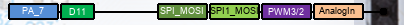
\includegraphics{images/nucleo_pin_functions.png}
\end{center}

Toutes les broches peuvent être utilisées en \textbf{entrée} ou en \textbf{sortie} \textbf{numérique}, c'est à dire un type de signal qui ne peut prendre que \textbf{deux états} : haut ou bas (aussi appelés 1 ou 0, ou encore \textit{HIGH} et \textit{LOW} en Arduino). 

\textit{Certaines broches ont également d'autres fonctionnalités : entrées analogiques, sorties modulées PWM, communication série...}

\subsection{Sorties numériques}

\subsubsection{Paramétrage}

Pour \textbf{configurer une broche en sortie}, il faut ajouter l'instruction suivante dans la fonction \textsl{setup()} (où \textsl{LED1} est le nom d'une broche du composant) :

\begin{lstlisting}
pinMode(LED1, OUTPUT);
\end{lstlisting}

\subsubsection{Utilisation}

Pour \textbf{affecter une valeur à une broche en sortie}, il faut utiliser une des deux instructions suivantes (où \textsl{LED1} est le nom d'une broche du composant) selon que l'on veut mettre la sortie à l'état bas (\textit{LOW}) ou à l'état haut (\textit{HIGH}) :

\begin{lstlisting}
digitalWrite(LED1, LOW);
digitalWrite(LED1, HIGH);
\end{lstlisting}


\subsection{Entrées numériques}

\subsubsection{Paramétrage}

Il n'y a aucun paramétrage à effectuer pour configurer une broche en entrée. Elles sont toutes \textbf{par défaut} paramétrer dans cette direction, notamment pour protéger les autres périphériques associés à la carte.

\subsubsection{Utilisation}

Pour \textbf{récupérer la valeur d'une broche en entrée}, il faut utiliser l'instruction suivante (où \textsl{SW1} est le nom d'une broche du composant) :

\begin{lstlisting}
bool valSw1 = digitalRead(SW1);
\end{lstlisting}

La variable \textsl{valSw1} contient alors l'état de l'entrée \textsl{SW1} et peut valoir \textit{\textbf{true}} (état logique haut) ou \textit{\textbf{false}} (état logique bas).

\subsection{Scrutation}

La \textbf{scrutation} (ou \textit{polling} en anglais) est une méthode de \textbf{vérification régulière de l'état des périphériques ou des capteurs} dans un système embarqué pour détecter si un événement spécifique s'est produit. 

Dans ce contexte, le programme principal exécute une boucle continue (fonction \textsl{loop()} sous Arduino) où il interroge périodiquement chaque périphérique pour voir s'il nécessite une action. 

\begin{center}
	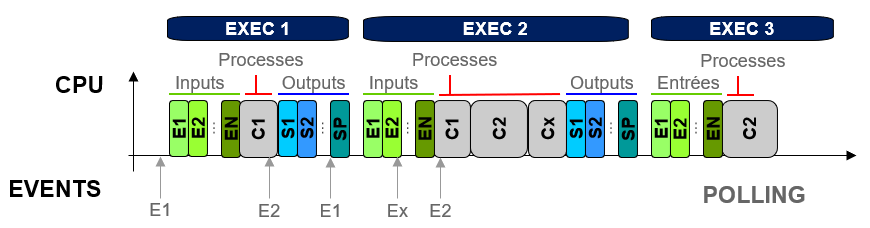
\includegraphics[width=0.8\textwidth]{images/gen_polling.png}
\end{center}

La \textbf{scrutation} ne permet pas de gérer d'un évènement rapidement et monopolise le microcontrôleur pour vérifier constamment l'état des capteurs ou des périphériques.


\subsection{Interruptions}

Une \textbf{interruption} est un signal envoyé au microcontrôleur pour lui demander d'\textbf{arrêter temporairement l'exécution de son programme principal} et de \textbf{s'occuper d'une tâche prioritaire spécifique}. Lorsque l'interruption est terminée, le microcontrôleur reprend son programme là où il s'était arrêté.

\begin{center}
	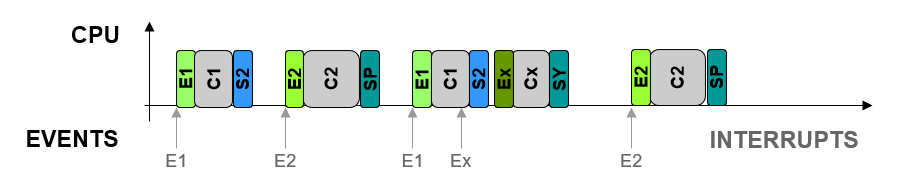
\includegraphics[width=0.8\textwidth]{images/gen_isr.png}
\end{center}


Cette méthode permet au système de \textbf{réagir rapidement à des événements externes} - changement de signal sur une broche, compteur qui atteint une certaine valeur - sans avoir besoin de vérifier constamment si l'événement a eu lieu, contrairement à la scrutation. 

Pour en savoir plus sur les interruptions, vous pouvez consulter le document à l'adresse suivante :

\href{https://iogs-lense-training.github.io/nucleo-basics/contents/polling_interrupts_rtos.html}{https://iogs-lense-training.github.io/nucleo-basics/contents/polling\_interrupts\_rtos.html}

\textit{Les interruptions sont également souvent utilisées dans les applications où un timing précis est nécessaire (par exemple, un compteur de temps).}


\subsubsection{Paramétrage}

Pour \textbf{configurer une broche en entrée permettant une interruption}, il faut ajouter l'instruction suivante dans la fonction \textsl{setup()} (où \textsl{LED1} est le nom d'une broche du composant) :

\begin{lstlisting}
pinMode(SW1, INPUT_PULLUP);
attachInterrupt(digitalPinToInterrupt(SW1), swInt, FALLING); 
\end{lstlisting}

Il existe 3 modes possibles pour les interruptions sur des signaux externes (entrées numériques) : 

\begin{itemize}
	\item \textbf{RISING} - front montant d'un signal
	\item \textbf{FALLING} - front descendant d'un signal
	\item \textbf{CHANGE} - fronts montant et descendant d'un signal
\end{itemize}


\subsubsection{Routine d'interruption}

Une \textbf{routine d'interruption}, aussi appelée \textbf{ISR} (\textit{Interrupt Service Routine}), est la fonction qui s'exécute automatiquement en réponse à une interruption. 

C'est une fonction classique, mais qui ne retourne pas de donnée.

\begin{lstlisting}
void swInt(void){
  bool ledState = digitalRead(LED1);
  digitalWrite(LED1, !ledState);
} 
\end{lstlisting}

Dans cet exemple, à chaque front descendant sur l'entrée \textsl{SW1}, la fonction \textsl{swInt()} est appelée. Elle lit alors l'état de la sortie \textsl{LED1} pour ensuite l'inverser.

\newpage
%%%%%%%%%%%%%%%%%%%%%%%%%%%%%%%%%%%%%%%%%%%%%%%%
%%%%%%%%%%%%%    Entrées analogiques et échantillonnage
\section{Liaison Série et débogage}

Lorsqu'on développe une \textbf{application sur un ordinateur}, il est facile de rajouter des lignes supplémentaires pour afficher des informations de débogage : soit sur une console, soit dans une partie de l'interface graphique développée.

En \textbf{programmation embarquée}, le microcontroleur n'a pas accès à un écran pour pouvoir communiquer facilement ce type d'informations. Il est donc plus difficile de connaître l'état de progression d'exécution du programme ou la valeur d’une variable à un moment donné du programme.

Il existe deux techniques permettant de répondre à cette attente :

\begin{itemize}
	\item à l'aide d'une sortie externe et d'un oscilloscope (et/ou d'une LED)
	\item à l'aide d'une liaison série entre la carte et l'ordinateur et d'un logiciel pour communiquer sur ce type de liaison
\end{itemize}

Nous allons nous intéresser ici à la seconde méthode, la première méthode proposée ne permettant pas de connaître la valeur d'une variable à un instant donné dans le programme.

\subsection{Liaison Série}

Pour connaître la valeur d'une variable à un instant donné dans le programme ou tout simplement afficher un message à l'utilisateur, nous allons nous servir d'une \textbf{liaison série de type RS232}, disponible sur les ordinateurs (par l'intermédiaire de la liaison USB pour Arduino) et sur la plupart des microcontroleurs.

Sur une liaison de type RS232, les données sont envoyées un bit à la fois en une seule file, ce qui rend la communication série simple et fiable pour les longues distances. Les données sont envoyées par \textbf{paquet de 8 bits} (soit un octet).

La transmission est \textbf{asynchrone} et les deux noeuds qui communiquent par ce protocole doivent donc accorder leur vitesse de transmission (\textit{baud rate} en anglais). Sur Arduino, on utilise couramment des vitesses comme 9600 bauds, 57600 bauds ou 115200 bauds.


\subsubsection{Paramétrage}

Par défaut, la liaison série configurée est celle utilisée par l'ordinateur (liaison émulée par le câble USB).

Lors de l'initialisation, il faut préciser la vitesse de transfert (en bauds).

\begin{lstlisting}
Serial.begin(9600);
while(!Serial);
\end{lstlisting}


\subsubsection{Envoi de données}

\begin{lstlisting}
Serial.print("LEnsE !");
\end{lstlisting}

\begin{lstlisting}
Serial.println(val_pot_m);
\end{lstlisting}

\subsubsection{Réception de données}

\subsection{Moniteur Série Arduino}

\newpage
%%%%%%%%%%%%%%%%%%%%%%%%%%%%%%%%%%%%%%%%%%%%%%%%
%%%%%%%%%%%%%    Entrées analogiques et échantillonnage
\section{Entrées analogiques et échantillonnage}

\subsection{Acquisition d'un échantillon}

où \textsl{POT\_IN} est le nom d'une broche du composant correspondant à une entrée analogique :

\begin{lstlisting}
int analogValue = analogRead(POT_IN);
\end{lstlisting}

La fonction \textsl{analogRead()} renvoie une valeur entière entre 0 et 1023 (10 bits), correspondant à la quantification de la tension présente sur la broche d'entrée analogique passée en paramètre.

Cette valeur, sur les cartes Nucléo, vaut : $$N = \frac{V_{in}}{3.3\operatorname{V}} * 1023$$

Il est alors possible d'afficher cette tension à l'aide de la liaison série :

\begin{lstlisting}
Serial.print("Pot = ");
Serial.println(analogValue);
\end{lstlisting}

Et si l'on veut afficher la valeur associée de la tension :

\begin{lstlisting}
Serial.print("Pot = ");
Serial.print(analogValue * 3.3 / 1023);
Serial.println(" V");
\end{lstlisting}

\textbf{Attention !} L'envoi de données sur la liaison série, pour l'affichage des valeurs par exemple, prend du temps ! Ce temps dépend bien entendu de la taille du message à transmettre mais également de la vitesse de transmission utilisée sur la liaison série.

\subsection{Echantillonnage à intervalle régulier}


\subsubsection{Paramètrage}

\begin{lstlisting}
#if defined(TIM1)
  TIM_TypeDef *Instance = TIM1;
#else
  TIM_TypeDef *Instance = TIM2;
#endif
  HardwareTimer *MyTim = new HardwareTimer(Instance);
  MyTim->setOverflow(10, HERTZ_FORMAT); // 10 Hz
  MyTim->attachInterrupt(samplingIsr);
  MyTim->resume();
\end{lstlisting}

Dans l'exemple précédent, la fonction \textsl{samplingIsr()} est appelée à intervalle régulier, ici à $10\operatorname{Hz}$.

\subsubsection{Routine d'interruption}

\begin{lstlisting}
int analogValue = 0;
bool samplingOk = false;
\end{lstlisting}


\begin{lstlisting}
void samplingIsr(){
  analogValue = analogRead(POT_IN);
  samplingOk = true;
}
\end{lstlisting}


\begin{lstlisting}
void loop() {
  if(samplingOk == true){
    Serial.print("Pot = ");
    Serial.println(valPot);
    samplingOk = false;
  }
}
\end{lstlisting}


\newpage
%%%%%%%%%%%%%%%%%%%%%%%%%%%%%%%%%%%%%%%%%%%%%%%%
%%%%%%%%%%%%%    Sorties modulées en largeur d'impulsion (PWM)
\section{Sorties modulées en largeur d'impulsion (PWM)}


\subsection{Pilotage de la luminosité d'une LED}


\subsection{Servomoteur}


\subsection{Branchement alternatif - STM32}

Toutes les sorties PWM des cartes Nucléo ne sont \textbf{pas nativement configurées pour fonctionner avec Arduino}. On parle de \textbf{broches alternatives} (ou fonctions alternatives sur certaines broches).

Si on souhaite pouvoir les utiliser avec Arduino, il est indispensable de rajouter une ligne de configuration dans la fonction \textsl{setup()} :

\begin{lstlisting}
LL_GPIO_SetAFPin_0_7(GPIOB,  GPIO_PIN_7,  GPIO_AF2_TIM4);
\end{lstlisting}

Cette ligne permet de modifier le paramétrage de la broche \textbf{PB7} afin qu'elle puisse fonctionner en PWM (ou avec la bibliothèque \textsl{Servo.h}.


\newpage
%%%%%%%%%%%%%%%%%%%%%%%%%%%%%%%%%%%%%%%%%%%%%%%%
%%%%%%%%%%%%%    I2C et SPI
\section{Liaisons I2C et SPI}

\subsection{Protocole I2C}

\subsubsection{Principe}

\subsubsection{Liaison physique}

\subsubsection{Mise en place sous Arduino}




\newpage
\subsection{Protocole SPI}

\subsubsection{Principe}

\subsubsection{Liaison physique}

\subsubsection{Mise en place sous Arduino}

%%%%%%%%%%%%%%%%%%%%%%%%%%%%%%%%%%%%%%%%%%%%%%%%
%%% RESSOURCES COMPLEMENTAIRES		


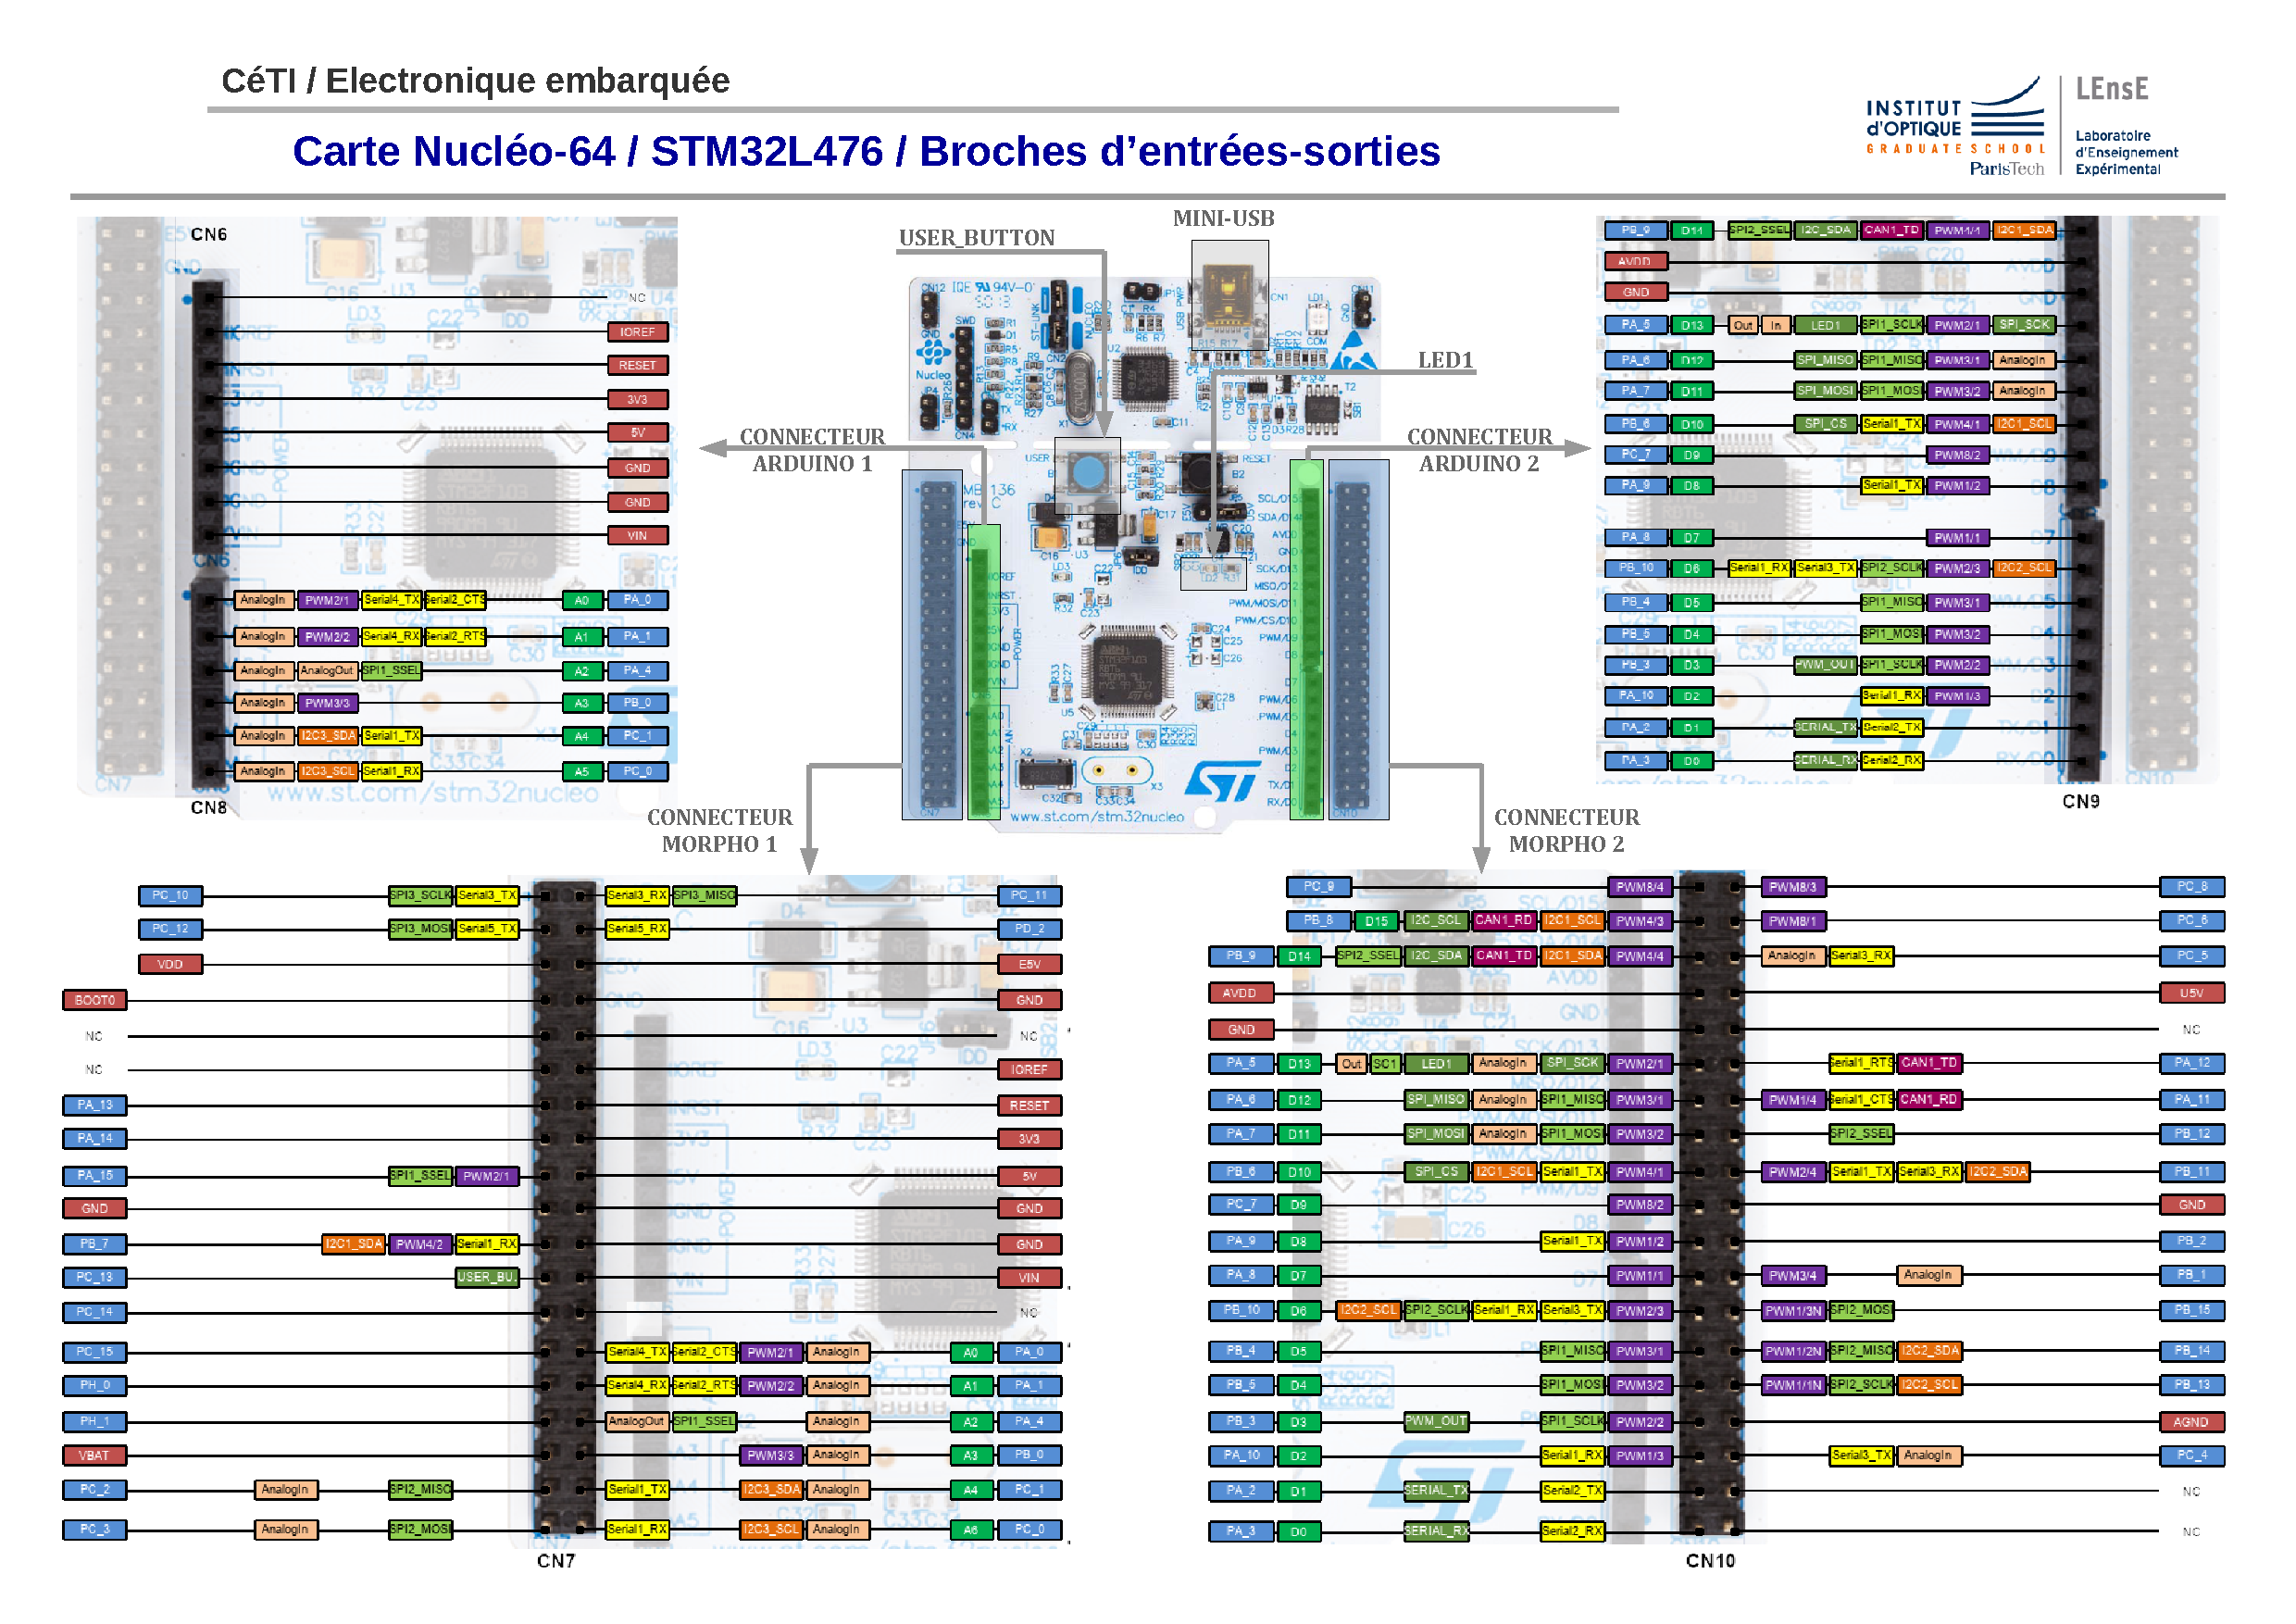
\includepdf[pages=1, landscape=true, pagecommand={\section{\texorpdfstring{\hspace{-1em}}{Brochage Nucléo L476RG}}}\label{doc:nucleo_pins_476RG}]{ressources/2021_FR_NucleoL476RG.pdf}

\end{document}


